% Skriv en kort text innan subsectionerna 
\subsection{Pixel size, magnification and resolution}
To take images of an object we used a CCD camera and the m-file \texttt{takeImage.m} which gave us black and white images. In background of the object we had a test chart with horizontal and vertical lines with different distances between their lines. 

We used these images and MatLab functions such as \texttt{imcrop, size} and \texttt{getpts} to calculate how many pixels on the screen that corresponded to a centimetre, determine a distance in the image and also to compare vertical and horizontal resolution. 

\subsection{Grey scale images, image format and image information}
We started by loading the image and normalizing the intensity by dividing it by 255. Then we use the \texttt{imcrop} command to select the part of the image we want to use. We then test some different functions to show that we can show the image in different ways, such as the \texttt{flipud} command to flip the image upside down. 

After we got comfortable with the different commands and understood how we could manipulate the image we moved on to the next part of the assignment and made two new matrices from the image. The first matrix, lets call this I1, we removed the first row and in the second matrix, we will call this I2, we removed the last row. I1 now have shifted one pixel.
By using the test chart we determine the MTF-values by summing along the columns on a arbitrary row.

\subsection{Image enhancement}
We try to enhance two images (see figure \ref{fig:histeqBefore}) with histogram equalization and contras stretching by using MatLab function \texttt{histeq} and \texttt{imhist}. 

\begin{figure}
	\centering
	\begin{subfigure}[b]{0.4\textwidth}
		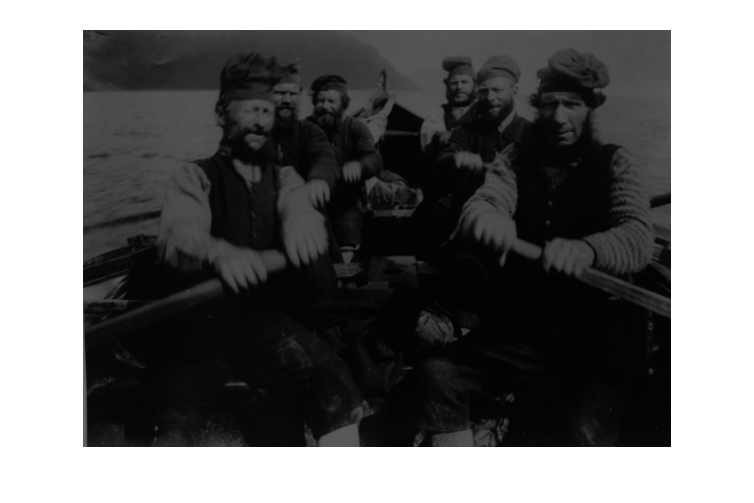
\includegraphics[width=\textwidth]{IE_img1org}
	\end{subfigure}
	\begin{subfigure}[b]{0.4\textwidth}
		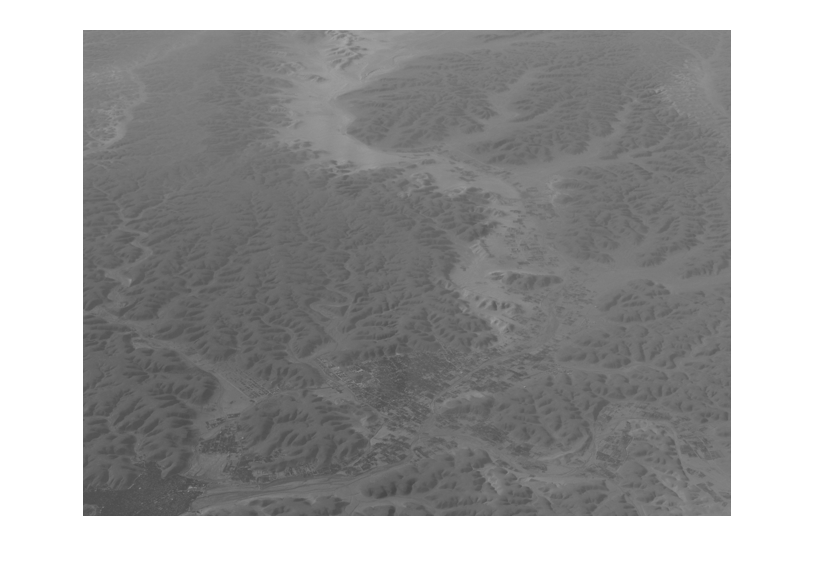
\includegraphics[width=\textwidth]{IE_img2org}
	\end{subfigure}
	\caption{Images used to enhance with histogram equalization.}
	\label{fig:histeqBefore}
\end{figure}

\subsection{Colour images}
We took a colour photo using a camera and transferred it to the computer and examined the resolution. We then used the MatLab command \texttt{imhist} to compare the spectrum of different parts of the image. % Kanske ska se över denna meningen lite
We also studied a method that if we selected the tomato it would highlight all red content in the image.

\subsection{IR - Imaging}
We use an infra-red camera to study heat conduction, friction heat and evaporation heat. We also study the transmission, reflection, absorption and scattering properties of some objects such as water, glass, plastic and whiteboard.